\chapter{骨关节炎风险预测模型构建}
第二章我们获取了骨关节炎患者的基因型数据并对其进行了预处理与特征筛选。本章则主要对骨关节炎风险预测模型做以介绍。该模型首先根据基于变分期望最大化算法的图估计器构建了输入基因型数据的关联并通过图来表示该关联关系。
之后构建了图神经网络对建立的图进行学习与处理并最终完成图的分类。该模型还通过融合患者表型进一步增强模型性能。最后本模型还构建了基于预测值与输入数据的模型解释器。
\section{图估计器}
\subsection{图神经网络中无结构数据的处理方法}
图神经网络只适用于图类型的数据,对常见无结构数据(例如文本,图像)的处理较为困难。本文目前获得的基因型数据也属于无结构数据,原理上不适用于图神经网络。
但是,考虑到图神经网络优秀的性能与可解释性,我们需要基于该无结构基因型数据构建图,继而输入图神经网络。目前根据无结构数据建图的方法主要有两种方法:
一种是通过分析数据构建静态图,神经网络训练过程中不对该图结构加以更新\cite{hu_embedding_2017,monti_geometric_2016},例如在处理无结构的图像数据时
,Monti\cite{monti_geometric_2016}提出了一种通过超像素将图像数据转为图的方法,使得图神经网络能够处理图像数据;第二种是通过学习方法构建动态图结构,
并在网络训练过程中不断更新图结构\cite{zhu_survey_2022}。这类通过学习方法获取图结构特征的过程也被称为图结构学习(Graph Structure Learning,GSL)。
目前的图结构学习过程主要分为三个步骤:首先通过已知数据通过k近邻法\cite{preparata_computational_1985}或者阈值法\cite{bentley_complexity_1977}
构建出一个初始图结构或观测图结构;然后使用诸如随机块模型(Stochastic Block Model,SBM)等方法\cite{holland_stochastic_1983}对该观测图结构进行建模;
最后通过算法估计出数据可能具有的图结构。在图估计的过程中,基于统计学的算法受到了广泛关注:例如Zhang\cite{zhang_bayesian_2019}等人提出了一种基于贝叶斯思想的图估计器。
其认为图结构根据依赖一定参数的分布所产生,如果通过蒙特卡洛方法对该参数进行估计,就可因此得到该分布的具体信息,继而对图结构进行估计。
Elinas\cite{elinas_variational_2020}同样基于贝叶斯思想提出了一种使用变分推断法的图估计方法。但是,以上研究仅适用于图神经网络中的节点分类问题,
同本研究所属图分类问题不符,不能直接应用于本研究中。但考虑到这类贝叶斯方法思路简洁,原理清晰。因此,本文也将基于贝叶斯思想构建适用于本文图分类问题的图结构估计器。

\subsection{问题描述}
贝叶斯思想认为:事件的观测值并不能反映事件的真实特性。贝叶斯方法因此主要解决由事件观测值向事件真实值的推断过程。
但是在讨论推断过程前,我们首先需要对观测值与真实值加以定义。
\subsubsection{观测值构建}
对于本文研究对象基因型数据而言,未经图神经网络处理的原始数据所含信息量较少,较难依据初始数据构建观测值。
但是有研究显示,经过谱图神经网络处理之后,具有较强关联的节点具有相似的值。\cite{hamilton_inductive_2018} 
我们因此认为在图神经网络的输出值中,对任一节点,如果有一其他节点与其有着相似的值,则两节点之间可能存在关联。
这种关联可以通过k近邻算法\cite{preparata_computational_1985}计算从而得到k近邻网络,而该k近邻网络可以很好地描述节点的局部特征。
在Wang\cite{wang_graph_2021}等人的研究中,也有通过根据图神经网络输出值构建k近邻网络的描述。
我们因此根据每个样本经图神经网络处理后的输出值建立k近邻网络,再将所有网络相加求平均以获得单个观测值。
同时为了防止信息丢失,我们将首次经图神经网络处理时输入的图初始化为全连接图,即认为每个节点都同其他节点存在关联。

\subsubsection{真实值构建}

本研究中所感兴趣的真实值为实际的未知图结构。但是对图结构的直接计算过于复杂,我们因此需要将图结构参数化,即使用少数几个参数来描述图结构。
目前在图论领域常用的图参数化模型为随机块模型\cite{holland_stochastic_1983},该模型认为图中的节点属于某几个簇,
节点之间是否相连仅与两节点所在的簇相关且服从某一参数化分布。
因此我们只需要得出支配该分布的参数就能对图结构加以复现,继而用少数参数描述庞大的网络。
因此本文将该类参数作为推断的目标,而由其产生的图结构作为模型输出值。

\subsubsection{推断过程}

界定了观测值与真实值之后,我们便可对图估计器所解决的问题加以严谨描述。

图估计器首先根据式\ref{equ:def_of_observation}有图神经网络的输出构建观测值$O$。

\begin{equation}\label{equ:def_of_observation}\begin{aligned}
    O^{ij}=\frac{1}{N}\sum_N o^{ij}_n
\end{aligned}\end{equation}

其中$O^{ij}$描述了节点$i,j$之间关联的观测值,$N$为样本数,$o^{ij}_n$为由第$n$个样本神经网络输出值构建的k近邻网络中节点$i,j$之间的关联。
通过该观测值我们构建图$G=(V,O)$,其中$V=\{v_1,...v_n\}$描述图中节点,即样本SNP位点。

为了通过SBM模型参数化图结构,我们假定图中共含有$C$个簇,每个节点$i$从属于簇$m$的概率由式\ref{equ:def_of_z_element}来描述,且$z_i$相互独立并满足由式\ref{equ:def_of_z}所描述的多项分布。

\begin{equation}\label{equ:def_of_z_element}
  z_{im}\in \bold{Z}^{N\times C},i\in \{1, ... ,n\},m\in\{1,...,C\}
\end{equation}

\begin{equation}\label{equ:def_of_z}
  \begin{aligned}
    z_i \mathop{\sim}^{iid} M(1,\alpha)
  \end{aligned}
\end{equation}

基于此,我们使用$z_i$来描述节点之间关联。我们认为任意两节点之间的关联相互独立并满足如式\ref{equ:o|z}所描述二项分布。

\begin{equation}\label{equ:o|z}
  \begin{aligned}
    o_{ij}|z_{im},z_{jn} = 1 \sim B(1,\pi_{z_iz_j})
  \end{aligned}
\end{equation}


可以看出,只要解出参数$\pi$与$\alpha$,就可以此构建出如图\ref{fig:SBM}所示的SBM模型,继而对图结构加以推断;因此本文给出以下目标:

\begin{figure}[!ht]
  \centering
  \includegraphics[width=7cm]{./figures/Chapter3/SBM.png}
  \caption{随机块模型及其参数化示意图} \label{fig:SBM}
\end{figure}

基于观察到的节点关联信息$O$以及隐变量$Z$,通过式\ref{equ:target}估计参数$\theta=\{\alpha,\pi\}$,并根据该参数给出推断图结构

\begin{equation}\label{equ:target}
  \begin{aligned}
    \hat{\theta}=\mathop{\arg\max} l_\theta(O)
  \end{aligned}
\end{equation}

\subsection{基于变分期望最大化的图估计}

\subsubsection{推导与整理}

在节点关联与节点簇信息均已知的情况下,我们首先由式\ref{equ:comp_of_observation_likelihood}计算似然函数$l_{\theta}$,根据边缘概率公式,有
\begin{equation}\label{equ:comp_of_observation_likelihood}
  \begin{aligned}
    l_\theta(O)=\sum_{Z}\log p_\theta(O,Z)=\sum_Z(\log p_{\pi}(O|Z) +\log p_\alpha(Z))
  \end{aligned}
\end{equation}

其中 
\begin{equation}\label{equ:comp_of_observation_likelihood1}
  \begin{aligned}
\sum_Z(\log p_{\pi}(O|Z)+\log p_\alpha(Z))=\sum_Z(\sum_{i,j}^{n}\sum_{m,n}^C\log p_\pi(o_{ij}|z_{im}z_{jn})
+\sum_{i}^N\sum_m^C\log p_\alpha(z_{im}))
  \end{aligned}
\end{equation}

给定参数时,有 

\begin{equation}\label{equ:comp_of_observation_likelihood2}
  \begin{aligned}
p_\pi(o_{ij}|z_{im}z_{jn};\pi)=\binom{1}{O_{ij}}[\pi_{mn}(1-\pi_{mn})^{1-O_{ij}}]^{ z_{im}z_{jn}}
  \end{aligned}
\end{equation}

\begin{equation}\label{equ:comp_of_observation_likelihood3}
  \begin{aligned}
p_\alpha(z_{im})=\alpha_m^{z_{im}} 
  \end{aligned}
\end{equation}

将式\ref{equ:comp_of_observation_likelihood2}与\ref{equ:comp_of_observation_likelihood3}代入式\ref{equ:comp_of_observation_likelihood1}可得式\ref{equ:full_likelihood}。

\begin{equation}\label{equ:full_likelihood}
  \begin{aligned}
l_\theta(O;\theta) &= \sum_Z(\sum_{i,j}^{n}\sum_{m,n}^C\log p_\pi(o_{ij}|z_{im}z_{jn})+\sum_{i}^N\sum_m^C\log p_\alpha(z_
{im}))\\ &=\sum_Z(\sum_{i,j}^{n}\sum_{m,n}^C\log \binom{1}{O_{ij}}[\pi_{mn}(1-\pi_{mn})^{1-O_{ij}}]^{ z_{im}z_{jn}}+\sum_
{i}^N\sum_m^C\log\alpha_m^{z_{im}})
  \end{aligned}
\end{equation}

\subsubsection{期望最大化算法}

考虑到似然函数中含隐变量$Z$,通常我们采用期望最大化算法\cite{dempster_maximum_1977}计算使得似然函数取极大的参数。我们对似然函数式\ref{equ:comp_of_observation_likelihood}做如下处理

\begin{equation}\label{equ:dealed_likelihood}
  \begin{aligned}
    l(O;\theta)=\log p(O;\theta)\\
&=\log \int_Zp(O,Z;\theta)dz\\
&=\log \int_Z q(Z)\frac{p(O,Z;\theta)}{q(Z)}dz\\
&=\log \mathop{\mathbb{E}}[\frac{p(O,Z;\theta)}{q(Z)}]
  \end{aligned}
\end{equation}


其中$q(Z)$为一辅助函数且满足$\int q(Z)=1$。根据Jensen不等式\cite{jensen_sur_1906},对任意一凸函数,有

\begin{equation}\label{equ:Jensen}
  \begin{aligned}
    \mathop{\mathbb{E}}[f(x)]\leq f(\mathop{\mathbb{E}}[x])
  \end{aligned}
\end{equation}

当且仅当$x=\mathop{\mathbb{E}}[x]$时等号成立。又因为$\log x$ 为一凸函数,因此将式\ref{equ:Jensen}代入式\ref{equ:dealed_likelihood},有

\begin{equation}\label{equ:jensen_in_likelihood}
  \begin{aligned}
l(O;\theta)=\log p(O;\theta)\\
&=\log \mathop{\mathbb{E}}[\frac{p(O,Z;\theta)}{q(Z)}]\\
&\geq  \mathop{\mathbb{E}}[\log\frac{p(O,Z;\theta)}{q(Z)}]
\end{aligned}\end{equation}

当且仅当式\ref{equ:jensen_in_likelihood}满足式\ref{equ:equal_constraits}所示条件时等号成立。

\begin{equation}\label{equ:equal_constraits}
  \begin{aligned}
\frac{p(O,Z;\theta)}{q(Z)}=c
\end{aligned}\end{equation}

对式\ref{equ:equal_constraits}进行变化,有:

\begin{equation}\begin{aligned}
q(Z)=c\cdot p(O,Z;\theta)
\end{aligned}\end{equation}

又因为$\int q(Z)dz=1$,有:

\begin{equation}\begin{aligned}
\int_Z q(Z)dz=\int_Z c\cdot p(O,Z;\theta)dz=1\\
c=\frac{1}{\int_Zp(O,Z;\theta)dz}
\end{aligned}\end{equation}

因此:

\begin{equation}\label{equ:def_qz}
  \begin{aligned}
q(Z)=\frac{p(O,Z;\theta)}{\int_Zp(O,Z;\theta)dz}=\frac{p(O,Z;\theta)}{p(O;\theta)}=p(Z|O;\theta)
\end{aligned}\end{equation}

将式\ref{equ:def_qz}代回原不等式\ref{equ:jensen_in_likelihood},我们由式\ref{equ:def_of_Q}构造辅助函数$Q$。

\begin{equation}\label{equ:def_of_Q}
  \begin{aligned}
l(O;\theta) \geq  \mathop{\mathbb{E}}[\log\frac{p(O,Z;\theta)}{q(Z)}]=\int_Zp(Z|O;\theta)\log \frac{p(O,Z;\theta)}{p(Z|O;\theta)}dz=Q(\theta^{t+1};\theta)
\end{aligned}\end{equation}

显然,在取等条件成立时,$Q$为似然函数$l(O;\theta)$的下界。期望最大化算法因此首先计算给定预期参数$\theta$时下界$Q$的值,再通过优化参数$\theta$ 提高下界$Q$,通过不断迭代计算使得似然函数极大的参数$\hat{\theta}$。具体步骤描述如下:

\begin{itemize}
    \item E步骤:计算$Q(\theta^{t+1};\theta)$
    \item M步骤:优化参数$\theta$
\end{itemize}


但在下界$Q$的计算过程中我们由式\ref{equ:def_of_Q}设$q(Z)=p(Z|O;\theta)$,但是在本问题中,$p(Z|O;\theta)$过于复杂,无法计算,因此也无法完成后续步骤。我们需要采取其他方法来估计参数$\theta$。

\subsubsection{变分期望最大化}
\paragraph{变分推理}

变分推理是贝叶斯统计领域遇到无法计算的分布时常见的处理方法\cite{jordan_introduction_1999}。它通过构建辅助函数来模拟无法计算的分布,并通过优化过程使得辅助函数逐渐逼近真实分布。\cite{jaakkola_bayesian_2000}该方法与本文所处理问题较为契合,我们因此结合变分推理来处理期望最大化过程中无法计算的分布$p(Z|O;\theta)$。

\paragraph{证据下限与KL散度}

在进一步解释之前我们需要先对可能使用到的概念加以说明。在上一节中我们已经证明,根据Jensen不等式,含隐变量的似然函数具有一下界。我们将该下界定义为似然函数的证据下界(Evidence Lower Bound,ELBO)\cite{tzikas_variational_2008} 。其具有如式\ref{equ:def_of_ELBO}所示形式。

\begin{equation}\label{equ:def_of_ELBO}
  \begin{aligned}
l(O;\theta)
&=\log \int_Z q(Z)\frac{p(O,Z;\theta)}{q(Z)}dz\\
&\geq \int_Z q(Z) \log \frac{p(O,Z;\theta)}{q(Z)}dz\\
&=J(q(Z);\theta)
\end{aligned}\end{equation}

我们同时根据式\ref{equ:def_of_KL}定义似然函数与证据下界之间的差为分布$q(Z)$与分布$p(Z|O)$之间的KL散度(Kullback-Leibler divergence)。\cite{neal_view_1998}

\begin{equation}\label{equ:def_of_KL}
  \begin{aligned}
l(O;\theta) - \int_Z q(Z) \log \frac{p(O,Z;\theta)}{q(Z)}dz \\
&= \int_Zq(Z)\log p(O;\theta)dz- \int_Z q(Z) \log \frac{p(O,Z;\theta)}{q(Z)}dz\\
&=\int_Zq(Z;\theta)\log \frac{p(O;\theta)q(Z;\theta)}{p(O,Z;\theta)}dz\\
&=-\int_Zq(Z;\theta)\log \frac{p(Z|O;\theta)}{q(Z;\theta)}dz\\
&=KL(q(Z)||p(Z|O))
\end{aligned}\end{equation}

可以看出,该散度衡量了两分布间的差异,可以用于后续辅助函数的构造。
\paragraph{辅助函数构建}

基于变分推理思想,我们构建辅助分布$q_\psi(Z)$来模拟无法计算的$p(Z|O)$。基于期望最大化思想,我们构建如式\ref{equ:construct_l_function}所示似然函数。

\begin{equation}\label{equ:construct_l_function}
  \begin{aligned}
l(O;\theta)=J(q_\psi(Z);\theta)+KL(q_\psi(Z)||p(Z|O))
\end{aligned}\end{equation}

式\ref{equ:construct_l_function}中首项描述了在使用辅助分布替换$p(Z|O)$时原始似然函数的下界,第二项描述了辅助分布与原始分布之间的差值。值得注意的是,KL散度具有非负性,即$KL(\cdot||\cdot)\geq 0$。我们因此给出如式\ref{inequ:lb_of_cons_l}所示不等式。

\begin{equation}\label{inequ:lb_of_cons_l}
  \begin{aligned}
l(O;\theta)\geq J(q_\psi(Z);\theta)
\end{aligned}\end{equation}

借助期望最大化思想,我们如果能够通过迭代计算辅助函数与参数使得式\ref{inequ:lb_of_cons_l}中下界$J(q_\psi(Z);\theta)$不断升高,就能使得该似然函数最终取最大。展开该下界,得式\ref{equ:full_cons_l}。

\begin{equation}\label{equ:full_cons_l}
  \begin{aligned}
J(q_\psi(Z);\theta)&={} \int_Z q(Z) \log \frac{p(O,Z;\theta)}{q(Z)}dz\\
&={} \int_Z q(Z) \log p(O,Z;\theta)dz-\int_Z q(Z) \log q(Z)dz\\
&={} \int_Z q(Z) ( \sum_{i,j}^{n}\sum_{m,n}^C\log \binom{1}{O_{ij}}[\pi_{mn}(1-\pi_{mn})^{1-O_{ij}}]^{ z_{im}z_{jn}}+
\sum_{i}^N\sum_m^C\log\alpha_m^{z_{im}})dz\\
&-\int_Z q(Z) \log q(Z)dz\\
&={}\mathop{\mathbb{E}}_{q_\psi(Z)}[\sum_i^N\sum_m^Cz_{im}\log \alpha_m]-\sum_i^N\sum_m^C \mathop{\mathbb{E}}_{q_\psi(Z)}[z_{im}]\log \mathop{\mathbb{E}}_{q_\psi(Z)}[z_{im}]\\
&+\mathop{\mathbb{E}}_{q_\psi(Z)}[\sum_{i<j}^N\sum_{m,n}^Cz_{im}z_{jn}\log ( \binom{1}{O_{ij}}
\pi_{mn}(1-\pi_{mn})^{1-O_{ij}})]
\end{aligned}\end{equation}

此时,我们构造基于服从参数$\tau$的多项分布的辅助函数,使得该辅助函数满足式\ref{equ:constraits_of_aux_fun}。

\begin{equation}\label{equ:constraits_of_aux_fun}
  \begin{aligned}
q_\psi(Z)=\prod_i^N q_\psi(Z_i)=\prod_i^N M(Z_i,\tau)
\end{aligned}\end{equation}

对于该变分参数$\tau$,我们依据多项分布的性质给出如下限制条件$\tau \in [0,1]^C,\sum_m \tau_{im} =1$。可以看出,该参数同原始隐变量$Z$的意义相同,都描述了节点属于簇的概率。因此我们给出如式\ref{equ:tau_z_relation1}与\ref{equ:tau_z_relation2}所示关系。

\begin{equation}\label{equ:tau_z_relation1}
  \begin{aligned}
\tau_{im}=p(q_\psi(z_{im}=1))=\mathop{\mathbb{E}}_{q_\psi(Z)}[z_{im}]
\end{aligned}\end{equation}

\begin{equation}\label{equ:tau_z_relation2}
  \begin{aligned}
\tau_{im}\tau_{jn}=p(q_\psi(z_{im}=1,z_{jn}=1) =\mathop{\mathbb{E}}_{q_\psi(Z)}[z_{im}z_{jn}]
\end{aligned}\end{equation}

将式\ref{equ:tau_z_relation1}与\ref{equ:tau_z_relation2}代入式\ref{equ:full_cons_l},有式\ref{equ:tau_in_full_cons}所示形式。

\begin{equation}\label{equ:tau_in_full_cons}
  \begin{aligned}
J(O;\theta)=-\sum_i\sum_m\tau_{im} \log \tau_{im} +\sum_i\sum_m \tau_{im} \log \alpha_m \\+\sum_{i<j}^N\sum_{m,n}^C\tau_{im}\tau_{jn}\log ( \binom{1}{O_{ij}}\pi_{mn}(1-\pi_{mn})^{1-O_{ij}})
\end{aligned}\end{equation}

此时我们可以发现,虽然该下界的形式较为复杂,但是在给定辅助函数与参数的情况下依然能够给出结果,我们采用变分法的目的也就达到了。因此我们设计如下变分期望最大化算法。

\begin{itemize}
    \item VE步骤:固定参数$\theta$,根据$J$更新变分参数$\tau$,并计算更新参数后下界$J$的值
    \item M步骤:固定变分参数$\tau$,根据$J$更新参数$\theta$,直至收敛。
\end{itemize}

\paragraph{参数求解}

\paragraph*{VE步}此步骤中主要基于式\ref{equ:compu_of_tau_sim}根据式\ref{equ:compu_of_tau}求解变分参数$\tau$。

\begin{equation}\label{equ:compu_of_tau_sim}
  \begin{aligned}
\hat{\tau}=\mathop{\arg\max}_\tau J(O,\theta;\tau)
\end{aligned}\end{equation}

\begin{equation}\label{equ:compu_of_tau}
  \begin{aligned}
J(O,\theta;\tau)=-\sum_i\sum_m\tau_{im} \log \tau_{im} +\sum_i\sum_m \tau_{im} \log \alpha_m\\ +\sum_{i<j}^N\sum_{m,n}^C\tau_{im}\tau_{jn}\log ( \binom{1}{O_{ij}}\pi_{mn}(1-\pi_{mn})^{1-O_{ij}})
\end{aligned}\end{equation}

考虑到式\ref{equ:compu_of_tau}中的参数存在限制条件$\sum_m \tau_{im} =1$,我们采用拉格朗日乘数法\cite{haj_stochastics_2019}对该式加以计算得\ref{equ:lagrange_in_tau}。

\begin{equation}\label{equ:lagrange_in_tau}
  \begin{aligned}
L(J,\lambda)&={}J(O,\theta;\tau)+\lambda_i(\sum_m \tau_{im}-1)\\
&={}-\sum_i\sum_m\tau_{im} \log \tau_{im} +\sum_i\sum_m \tau_{im} \log \alpha_m+\lambda_i(\sum_m \tau_{im}-1)\\ &+\sum_{i<j}^N\sum_{m,n}^C\tau_{im}\tau_{jn}\log ( \binom{1}{O_{ij}}\pi_{mn}(1-\pi_{mn})^{1-O_{ij}})
\end{aligned}\end{equation}

将式\ref{equ:lagrange_in_tau}分别对$\tau_{im}$与$\lambda$求偏导,得式\ref{equ:partial_L_tau}与\ref{equ:partial_L_lambda}。

\begin{equation}\label{equ:partial_L_tau}
  \begin{aligned}
\frac{\partial L}{\partial \tau_{im}}=\sum_{j}^N\sum_{n}^C\tau_{jn}\log ( \binom{1}{O_{ij}}\pi_{mn}(1-\pi_{mn})^{1-O_{ij}})+\log \alpha_m -\log \tau_{im} +\lambda_i-1=0
\end{aligned}\end{equation}

\begin{equation}\label{equ:partial_L_lambda}
  \begin{aligned}
\frac{\partial L}{\partial \lambda_i}=\tau_{im}-1=0
\end{aligned}\end{equation}

对式\ref{equ:partial_L_tau}加以变换,我们得到式\ref{equ:compu_of_tau}。
\begin{equation}\label{equ:compu_of_tau}
  \begin{aligned}
\log \tau_{im} =\sum_{j}^N\sum_{n}^C\tau_{jn}\log ( \binom{1}{O_{ij}}\pi_{mn}(1-\pi_{mn})^{1-O_{ij}})+\log \alpha_m -\lambda_i+1
\end{aligned}\end{equation}

我们因此基于式\ref{equ:compu_of_tau}给出$\tau_{im}$的解析解

\begin{equation}\label{equ:solution_of_tau}
  \begin{aligned}
\tau_{im} = e^{-\lambda_i+1}\alpha_m[\prod_j^N\prod_n^C[ \binom{1}{O_{ij}}\pi_{mn}(1-\pi_{mn})^{1-O_{ij}}]^{\tau_{jn}}]\\
\forall i \in \{1 ...N\} ;\forall m \in \{1 ... C\}
\end{aligned}\end{equation}

可以看出,每个变分参数的计算都依赖于其他变分参数,虽然可以通过迭代至收敛的方法计算,但这也对参数初始值的选取提出了要求,具体细节将于后文讨论。

\paragraph*{M步}此步骤中主要基于式\ref{equ:compu_of_theta_sim}求解目标参数$\theta$。

\begin{equation}\label{equ:compu_of_theta_sim}
  \begin{aligned}
\hat{\theta}=\mathop{\arg\max}_\theta J(O,\tau;\theta)
\end{aligned}\end{equation}

首先我们根据式\ref{equ:J_theta}计算$\theta$中的$\pi$。由于$\pi$在式中相对较为独立,我们直接对其求偏导得式\ref{equ:partial_J_pi}。

\begin{equation}\label{equ:J_theta}
  \begin{aligned}
J(O,\tau,\alpha;\pi)=-\sum_i\sum_m\tau_{im} \log \tau_{im} +\sum_i\sum_m \tau_{im} \log \alpha_m\\ +\sum_{i<j}^N\sum_{m,n}^C\tau_{im}\tau_{jn}\log ( \binom{1}{O_{ij}}\pi_{mn}(1-\pi_{mn})^{1-O_{ij}})
\end{aligned}\end{equation}

\begin{equation}\label{equ:partial_J_pi}
  \begin{aligned}
\frac{\partial J(O,\tau,\alpha;\pi)}{\partial \pi_{mn}}=\sum_{i<j}\tau_{im}\tau_{jn}(\frac{O_{ij}}{\pi_{mn}}-\frac{1-O_{ij}}{1-\pi_{mn}})
\end{aligned}\end{equation}

求解以上方程,得如式\ref{equ:solution_pi}所示的$\pi$的解析解。

\begin{equation}\label{equ:solution_pi}
  \begin{aligned}
\hat{\pi_{mn}}=\frac{\sum_{i<j}\tau_{im}\tau_{jn}O_{ij}}{\sum_{i<j}\tau_{im}\tau_{jn}}
\end{aligned}\end{equation}

对于$\theta$中的$\alpha$,由于其也存在限制条件$\sum_m \alpha_m=1$,我们依旧采用拉格朗日乘数法计算得式\ref{equ:lagrange_in_alpha}。

\begin{equation}\label{equ:lagrange_in_alpha}
  \begin{aligned}
L(J,\lambda)&={}J(O,\pi,\tau;\alpha)+\lambda_i(\sum_m \alpha_{m}-1)\\
&={}-\sum_i\sum_m\tau_{im} \log \tau_{im} +\sum_i\sum_m \tau_{im} \log \alpha_m+\lambda_i(\sum_m \alpha_{m}-1)\\ &+\sum_{i<j}^N\sum_{m,n}^C\tau_{im}\tau_{jn}\log ( \binom{1}{O_{ij}}\pi_{mn}(1-\pi_{mn})^{1-O_{ij}})
\end{aligned}\end{equation}

将该式分别对$\alpha_{m}$与$\lambda$求偏导,得式\ref{equ:partial_L_alpha}与式\ref{equ:partial_L_lambda}。

\begin{equation}\label{equ:partial_L_alpha}
  \begin{aligned}
\frac{\partial L}{\partial \alpha_m}=\frac{\sum_i\tau_{im}}{\alpha_m}+\lambda_i=0
\end{aligned}\end{equation}

\begin{equation}\label{equ:partial_L_lambda}
  \begin{aligned}
\frac{\partial L}{\partial \lambda_i}=\alpha_{m}-1=0
\end{aligned}\end{equation}

对式\ref{equ:partial_L_alpha}加以处理,得:

\begin{equation}\begin{aligned}
\frac{\sum_i\tau_{im}}{\alpha_m}+\lambda_i&=0\\
\sum_i\tau_{im}+\alpha_m\lambda_i&=0\\
\sum_m\sum_i\tau_{im}+\sum_m\alpha_m\lambda_i&=0\\
\lambda_i=-\sum_m\sum_i\tau_{im}
\end{aligned}\end{equation}

代原式\ref{equ:partial_L_alpha},得如式\ref{equ:solution_alpha}所描述的$\alpha$的解析解。

\begin{equation}\label{equ:solution_alpha}
  \begin{aligned}
\hat{\alpha_m}&=\frac{\sum_i\tau_{im}}{\sum_m\sum_i\tau_{im}}\\
&=\frac{\sum_i\tau_{im}}{N}
\end{aligned}\end{equation}

至此,我们已经完成了所有参数的估计。确定参数后只需将其代回原始模型即可得出估计的节点之间关联,继而完成图结构的构建。

\subsubsection{起始与终止条件}

之前在对变分参数$\tau$的计算中我们发现,任一参数的计算都依赖于其他参数。但是如果以零为初始值,参数在计算时只会考虑项$e^{-\lambda_i+1}\alpha_m$,无法对参数$\pi$形成有效估计。
因此我们需要通过一定方法给予该变分参数初值,并通过迭代的方法计算$\tau$直至收敛。
目前的研究中常使用k-Means法\cite{haj_estimation_2020}先对节点进行聚类,根据聚类结果对变分参数进行赋值。
但是k-Means法需要预先确定图中节点簇数$C$,且对于一般问题而言该簇数未知,因此需要一种能够评估所选簇数对最终似然函数影响的方法。
目前研究中,一种叫做贝叶斯信息指标(Bayesian Information Criterion,BIC)\cite{schwarz_estimating_1978}的方法可以用来完成类似工作,其定义为式\ref{equ:BIC}。

\begin{equation}\label{equ:BIC}
  \begin{aligned}
    BIC(C)=\log P(O;\theta)-\frac{V_C}{2}\log N
\end{aligned}\end{equation}

其中$\log P(O;\theta)$描述对应模型下的似然函数,$V_C$描述了选择对应簇数$C$时模型参数数量,但是该方法涉及到无法求解似然函数的计算,在本研究中无法实现。但是,基于类似的思想,Daudin等人提出另一种评价指标:整合分类似然(Integrated Classification Likelihood,ICL)\cite{daudin_mixture_2008},该指标并不直接计算原始似然函数,而是通过计算变分时使用的变分似然函数给出评判依据。
该指标定义如式\ref{equ:ICL}。

\begin{equation}\label{equ:ICL}
  \begin{aligned}
ICL(C)=\sum_i\sum_m\tau_{im} \log \tau_{im} +\sum_{i<j}^N\sum_{m,n}^C\tau_{im}\tau_{jn}\log ( \binom{1}{O_{ij}}\pi_{mn}(1-\pi_{mn})^{1-O_{ij}})\\-\frac{1}{2}(\frac{C(C+1)}{2}\log \frac{N(N-1)}{2}-(C-1)\log N)
\end{aligned}\end{equation}

基于以上信息,我们给出图\ref{fig:Estimator}描述的基于变分期望最大化的图估计算法全流程。

\begin{figure}[!ht]
  \centering
  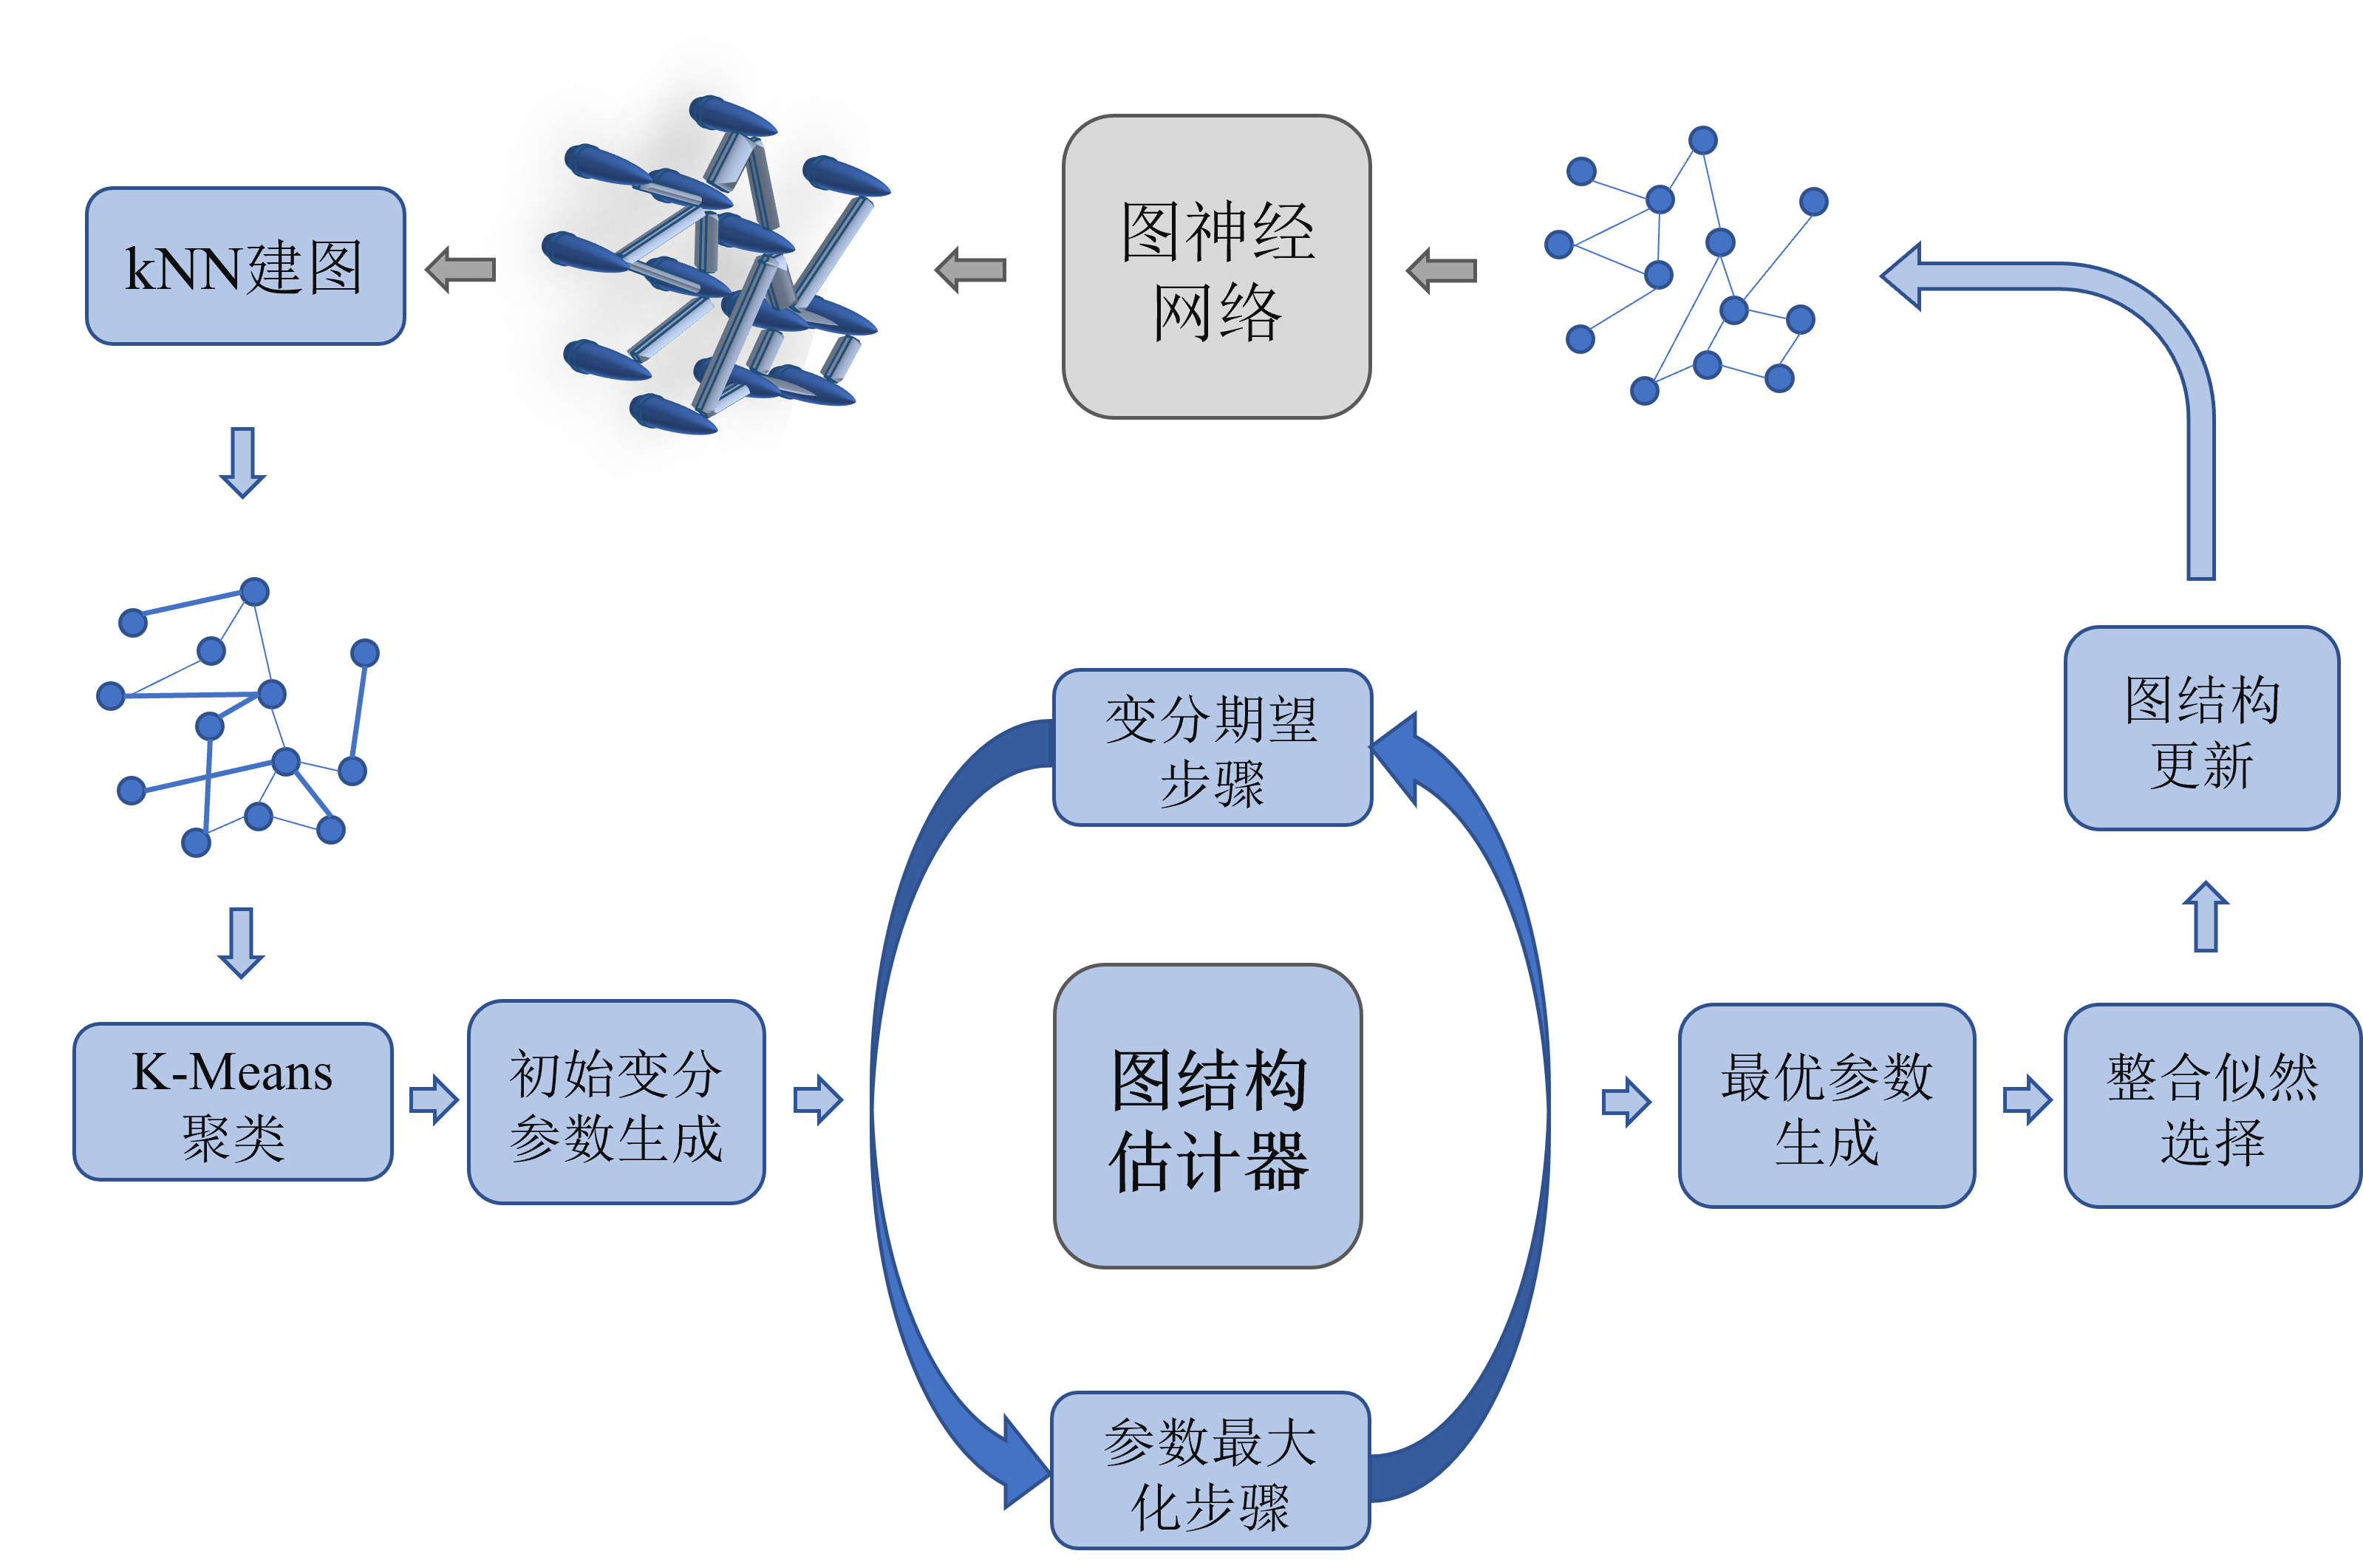
\includegraphics[width=\textwidth]{./figures/Chapter3/Estimator.png}
  \caption{基于变分期望最大化的图估计算法流程} \label{fig:Estimator}
\end{figure}

\begin{algorithm}
\label{algo:VEM}
\SetAlgoLined
\caption{基于变分期望最大化的图估计算法}
\KwData{观测值$O$与聚类数目$c$}
\KwResult{模型参数$\theta$}
\KwIn {观测值,确定簇数范围}

使用k-Means法对输入值进行聚类,给出初始变分参数$\tau_0$

\While{$\theta$不收敛}{
    VE步
    
        \While{变分参数$\tau$不收敛}{
             循环计算$\hat{\tau}=\mathop{\arg\max}_\tau J(O,\theta;\tau)$
             }
             
    根据该变分参数计算 $J$
    
    M步
    
    根据$\hat{\theta}=\mathop{\arg\max}_\theta J(O,\tau;\theta)$计算参数$\theta$
    
    计算最优似然下界$\hat{J}$与该簇数下的整合分类似然$ICL(C)$
}
\KwOut {选择使得整个分类似然最小的簇数$C$,选择该簇数计算出的参数$\hat\theta$}
\end{algorithm}

\section{图神经网络}
在完成了输入图结构的估计后,我们便可开始设计模型中图处理的核心——图神经网络。基于绪论中对图神经网络的讨论与综述,本文决定使用谱图神经网络中的切比雪夫层来处理生成的图数据。

\subsection{基本定义}

为了高效处理图数据,我们将图估计器所生成的节点关系通过矩阵表示,这类描述图节点之间关联的矩阵被称为邻接矩阵(Adjacency Matrix),用$A$来表示
\begin{equation}\begin{aligned}
A_{ij}=\{0,1\}^{N\times N}
\end{aligned}\end{equation}
$A_{ij}=1$意味着节点$i$,$j$之间存在相关,反之$A_{ij}$意味着两节点之间无相关关系。我们同时定义无向图中节点的度(Degree)为与该节点相关节点的数量并定义图的度矩阵$D$为
\begin{equation}\begin{aligned}
D_{ii}=\sum_{i\neq j}A_{ij}
\end{aligned}\end{equation}
可以看出,该度矩阵为一对角矩阵。同时为了后续矩阵的特征分解操作,我们定义图的拉普拉斯矩阵$L$为度矩阵与邻接矩阵之差,即
\begin{equation}\begin{aligned}
L=D-A
\end{aligned}\end{equation}
\subsection{切比雪夫层}

切比雪夫网络是一种谱图神经网络,其通过卷积方式来从数据中学习复杂信息\cite{proakis_digital_1996}。但是同常见的卷积神经网络不同,谱图神经网络通过傅里叶变换的方式来实现图这种非欧数据上的卷积。根据卷积定理\cite{stahlschmidt_multimodal_2022},两个函数的卷积为他们傅里叶变换后的结果的点积的傅里叶逆变换,即
\begin{equation}\begin{aligned}
x * y=F^{-1}\{F\{x\}\cdot F\{y\} \}
\end{aligned}\end{equation}
因此如果我们能够在图上定义一傅里叶变换,我们就能以此定义图数据上的卷积。通常来说,函数的傅里叶变换是函数在拉普拉斯算子特征函数这一组标准正交基上的投影。类似地,我们根据图的拉普拉斯矩阵定义该变换。
\begin{equation}\begin{aligned}
Lu=\lambda u
\end{aligned}\end{equation}
其中$L$为图的拉普拉斯量,$u$为该正交基,$\lambda$为特征值。我们同时定义矩阵$U=[u_1,...u_N]$,使得
\begin{equation}\begin{aligned}
L=U^T\Lambda U
\end{aligned}\end{equation}
因此我们定义图$\phi$上的傅里叶变换为
\begin{equation}\begin{aligned}
\hat \phi &=U^T\phi \\
&=diag(\hat \phi(\lambda_l))\\
&=diag(\sum_i^N\phi_iu_{li})
\end{aligned}\end{equation}
因此根据卷积定理,对于滤波器$g$与图信号$x$而言,在图$G$上定义的卷积为
\begin{equation}\begin{aligned}
(g*x)_{G}&=U(U^Tg\cdot U^Tx)\\
&=Ug_\theta(\Lambda) U^Tx\\
&=g_\theta(L)x
\end{aligned}\end{equation}
其中$g_\theta$为卷积核在图中的傅里叶变换,$\theta$为该卷积核的参数。因此我们可以定义谱图神经网络中的一层为
\begin{equation}\begin{aligned}
y=\sigma(g_\theta(L)x)
\end{aligned}\end{equation}
但是,此时$g_\theta$较难确定。Defferend[65]等人依靠切比雪夫多项式对$g_\theta$进行了近似,其认为
\begin{equation}\begin{aligned}
g_{\theta}(\Lambda)=\sum_{k=0}^{K}\theta_kT_k(\tilde{\Lambda}),\ \tilde{\Lambda}=2\Lambda_n/\lambda_{max}-I_n
\end{aligned}\end{equation}
其中$\theta$代表需要在训练中学习的参数,$T_k$代表$k$阶切比雪夫行列式,$\tilde{\Lambda}$代表特征矩阵。其中切比雪夫行列式计算方式如下。
\begin{equation}\begin{aligned}
T^{(0)} &= X \\
T^{(1)} &= \tilde L X \\
T^{(k \ge 2)} &= 2 \cdot \tilde L T^{(k - 1)} - T^{(k - 2)},
\end{aligned}\end{equation}
因此切比雪夫网络中的一层表示为
\begin{equation}\begin{aligned}
Y=\sigma \left(  \sum_{k=0}^{K-1}{\theta_k T_k (\tilde{L})}   x \right) 
\end{aligned}\end{equation}

\subsection{结构设计}

基于切比雪夫层的特点,我们构建如下图神经网络。

\begin{itemize}
\item
  切比雪夫层
\item
  切比雪夫层
\item
  读出层
\item
  全连接层
\end{itemize}

其中切比雪夫层设置阶数$k=1$,原理上该型卷积核同CNN中最经典的$3\times3$卷积核作用结果相仿。每层切比雪夫层会使节点融合与其相邻节点的信息,增强模型对局部信息的处理能力。读出层将进过行卷积操作的图再次转化为无结构数据,再将该数据输入全连接层中用以后续的风险预测。
\section{表型融合}
考虑到骨关节炎作为一种复杂多基因疾病,单纯以基因型为输入可能导致风险预测效果不佳。因此有必要同时融合表型数据。根据Boer\cite{boer_deciphering_2021}等人的报道,我们选择同骨关节炎密切相关的表型做为协变量并从UKB数据库中获取相关表型数据。具体表型如下表。
\begin{table}[!h]
	\renewcommand{\arraystretch}{1.2}
	\centering\wuhao
	\caption{选取协变量表型} \label{ICD_exclude} \vspace{2mm}
	\begin{tabularx}{\textwidth} { 
   >{\centering\arraybackslash}X 
   >{\centering\arraybackslash}X }
	\toprule[1.5pt]
		UKBID & 表型 \\
	\midrule[1pt]
		32883-31 & 性别 \\
        32883-48 & 髋围 \\
        32883-49 & 腕围 \\
        32883-2463 & 是否发生过骨折 \\
        32883-21001 & BMI \\
        32883-21002 & 体重 \\
        32883-21003 & 年龄 \\
	\bottomrule[1.5pt]
	\end{tabularx}
\end{table}
同时我们选择多模态数据融合中的中间融合法\cite{gaudillo_machine_2019}将基因型数据与表型数据相融合。我们将已构建的图神经网络的中间输出层与所获取的表型数据相融合,并输入新的分类器进行训练,最终给出融合表型后的预测结果。

\section{图解释器}
图是一种包含了节点信息与节点之间关系的数据结构,但是,本文目前为止建立的模型只能直接给出对患病风险的预测,与传统机器学习方法无异。如果能够充分利用图中的关联信息并对产生该预测结果的原因加以解释,不仅能够增强预测结果可信性,还能根据其解释内容发掘数据中潜藏的其他信息。目前对于图神经网络解释器的研究已有颇多进展,本文基于其中备受关注的GNNExplainer \cite{ying_gnnexplainer:_2019}来构建模型解释器。

GNNExplainer通过输入的已训练图神经网络模型及其预测结果从输入数据中选择对预测结果影响最大的子图。其数学描述如下
\begin{equation}\begin{aligned}
    \max_{Gs} MI (Y, G_S) = H(Y) - H(Y|G=G_S)
\end{aligned}\end{equation}

其中

\begin{itemize}
\item
  \(MI\)表示两变量之间的互信息(Mutual
  Information),其代表两变量之间相互依赖的程度。
\item
  \(Y\)表示模型给出的预测结果
\item
  \(G_s\)表示同预测结果相关的子图
\item
  \(H\)表示变量的信息熵
\end{itemize}

该文献描述:对于给定的GNN模型,$H(Y)$恒定,此时只需要最小化$ H(Y|G=G_S)$就可达到解释目的。该文献同时描述了一种变分近似方法来实现该优化过程,最终生成了与预测结果相关的最小子图。

\section{本章小结}
本章描述了骨关节炎风险预测模型的构建过程与基本模块。本文首先针对现存基因型数据结构缺失的问题基于变分期望最大化算法构建了一个图结构估计器。该估计器能根据神经网络的输出动态更新与预测图结构,同时能够对图中的节点聚类分析。其次,本文根据谱图神经网络中的切比雪夫层构建了包裹卷积层、读出层、全连接层在内的图神经网络用于图数据的处理以及患病风险的预测。考虑到单纯通过基因型数据预测患病风险结果可能较差,本文还基于文献描述的同骨关节炎密切相关的表型构建了表型融合风险预测模型。最后,为了尽最大可能挖掘出图数据中的潜藏信息,本文还根据已有的图神经网络解释器构建了预测结果解释器,在给出风险预测结果的同时获取同预测结果相关的子图。以上模块共同构成了本文预期的骨关节炎风险预测模型。 